%% LyX 1.6.5 created this file.  For more info, see http://www.lyx.org/.
%% Do not edit unless you really know what you are doing.
\documentclass[english]{article}
\usepackage[T1]{fontenc}
\usepackage[latin9]{inputenc}
\usepackage{graphicx}

\makeatletter

%%%%%%%%%%%%%%%%%%%%%%%%%%%%%% LyX specific LaTeX commands.
%% Because html converters don't know tabularnewline
\providecommand{\tabularnewline}{\\}

\makeatother

\usepackage{babel}

% The following can be used if not using custom frontpage
\title{<document title>}
\author{<name>\\
        \\
        <student id>
}
\date{\today}

\begin{document}

\section{Abstract}

\section{Specification analysis}

By studying the specification we conclude that we will be needing
eight different states; one for each {}``circle''. For input we
need a control for the direction (clockwise or counter-clockwise)
and a reset switch.

For output we would at minimum need to specify the orientation and
the number of the current circle to be displayed. These are defined
as top,d1,d0 (d for digit).\\
\\
Following the specification flow, leaves us with the following
finite state machine.


\subsection{Finite State Machine}

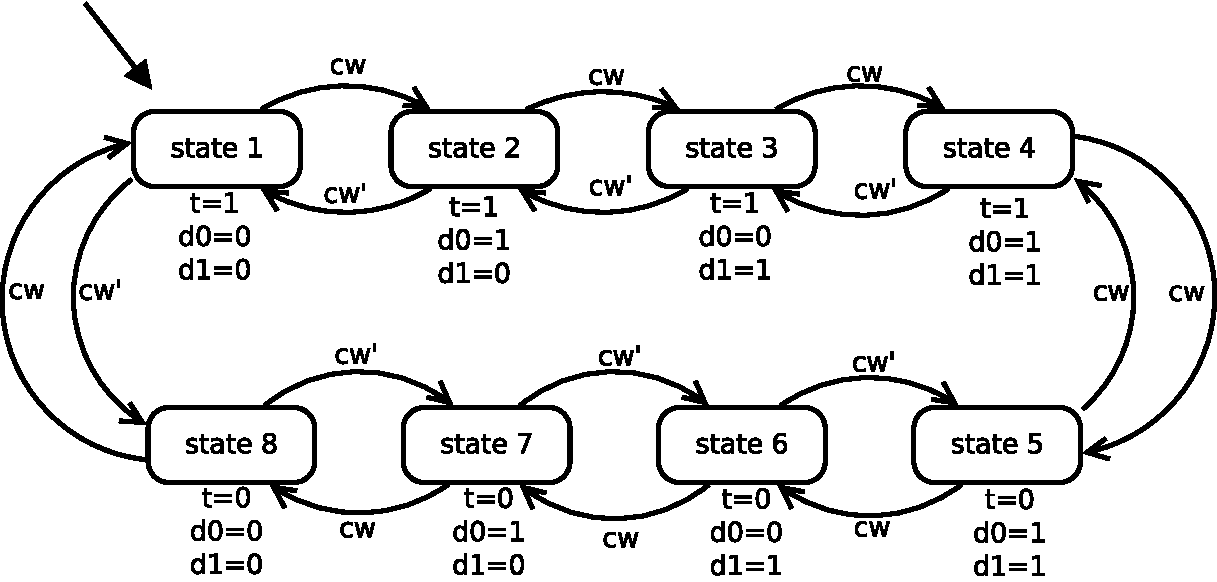
\includegraphics[width=0.7\textwidth]{fig/FSM_states}


\section{Truth table}

\begin{tabular}{cccc|cccccc}
s2 & s1 & s0 & cw & n2 & n1 & n0 & d1 & d0 & top\tabularnewline
\hline
\hline 
0 & 0 & 0 & 1 & 0 & 0 & 1 & 0 & 0 & 1\tabularnewline
\hline
0 & 0 & 1 & 1 & 0 & 1 & 0 & 0 & 1 & 1\tabularnewline
\hline 
0 & 1 & 0 & 1 & 0 & 1 & 1 & 1 & 0 & 1\tabularnewline
\hline 
0 & 1 & 1 & 1 & 1 & 0 & 0 & 1 & 1 & 1\tabularnewline
\hline 
1 & 0 & 0 & 1 & 1 & 0 & 1 & 1 & 1 & 0\tabularnewline
\hline 
1 & 0 & 1 & 1 & 1 & 1 & 0 & 1 & 0 & 0\tabularnewline
\hline 
1 & 1 & 0 & 1 & 1 & 1 & 1 & 0 & 1 & 0\tabularnewline
\hline 
1 & 1 & 1 & 1 & 0 & 0 & 0 & 0 & 0 & 0\tabularnewline
\hline 
0 & 0 & 0 & 0 & 1 & 1 & 1 & 0 & 0 & 1\tabularnewline
\hline 
0 & 0 & 1 & 0 & 1 & 1 & 0 & 0 & 1 & 1\tabularnewline
\hline 
0 & 1 & 0 & 0 & 1 & 0 & 1 & 1 & 0 & 1\tabularnewline
\hline 
0 & 1 & 1 & 0 & 1 & 0 & 0 & 1 & 1 & 1\tabularnewline
\hline 
1 & 0 & 0 & 0 & 0 & 1 & 1 & 1 & 1 & 0\tabularnewline
\hline 
1 & 0 & 1 & 0 & 0 & 1 & 0 & 1 & 0 & 0\tabularnewline
\hline 
1 & 1 & 0 & 0 & 0 & 0 & 1 & 0 & 1 & 0\tabularnewline
\hline 
1 & 1 & 1 & 0 & 0 & 0 & 0 & 0 & 0 & 0\tabularnewline
\hline
\end{tabular}


\subsection{Equations}


\subsubsection{n2}
$\left(s'_{2}s_{1}s_{0}+s_{2}s'_{1}s'_{0}+s'_{2}s_{1}s'_{0}+s_{2}s_{1}s'_{0}\right)cw'+\left(s'_{2}s_{1}s_{0}+s_{2}s'_{1}s'_{0}+s'_{2}s_{1}s'_{0}+s_{2}s_{1}s'_{0}\right)cw$ 

$\Leftrightarrow  s'_{2}s_{1}s_{0}+s_{2}s'_{1}s'_{0}+s'_{2}s_{1}s'_{0}+s_{2}s_{1}s'_{0}$

\subsubsection{n1}

$\left(s'_{2}s'_{1}s_{0}+s'_{2}s_{1}s'_{0}+s_{2}s'_{1}s_{0}+s_{2}s_{1}s'_{0}\right)cw'+\left(s'_{2}s'_{1}s_{0}+s'_{2}s_{1}s'_{0}+s_{2}s'_{1}s_{0}+s_{2}s_{1}s'_{0}\right)cw$

$\Leftrightarrow  s'_{2}s'_{1}s_{0}+s'_{2}s_{1}s'_{0}+s_{2}s'_{1}s_{0}+s_{2}s_{1}s'_{0}$


\subsubsection{n0}

$\left(s'_{2}s'_{1}s'_{0}+s'_{2}s_{1}s'_{0}+s_{2}s'_{1}s'_{0}+s_{2}s_{1}s'_{0}\right)cw'+\left(s'_{2}s'_{1}s'_{0}+s'_{2}s_{1}s'_{0}+s_{2}s'_{1}s'_{0}+s_{2}s_{1}s'_{0}\right)cw$

$<=> s'_{2}s'_{1}s'_{0}+s'_{2}s_{1}s'_{0}+s_{2}s'_{1}s'_{0}+s_{2}s_{1}s'_{0}$

\subsubsection{d1}
$D_{1}$ is by definition unaffected by the $cw$ variable. 
\begin{eqnarray*}
s_{2}'s_{1}s_{0}' + s_{2}'s_{1}s_{0} + s_{2}s_{1}'s_{0}' + s_{2}s_{1}'s_{0} & \Leftrightarrow\\
s_{2}'s_{1} + s_{2}s_{1}'
\end{eqnarray*}


\subsubsection{d0}
$D_{0}$ is by definition unaffected by the $cw$ variable. 

\begin{eqnarray*}
s_{2}'s_{1}'s_{0} + s_{2}'s_{1}s_{0} + s_{2}s_{1}'s_{0}' + s_{2}s_{1}s_{0}' & \Leftrightarrow\\
s_{2}'s_{0}+s_{2}s_{0}'
\end{eqnarray*}



\subsubsection{$t$}

By Studying the truth table it becomes apparant that $t$ is only
true when $s_{2}$ is false:

\begin{center}
$t = s_{2}'$
\par\end{center}


\section{Solution description}

\section{Tests}

\section{Conclusion}


\newpage

\appendix


\section{Appendix1}
\section{Appendix2}
\section{Appendix3}

\end{document}
